\documentclass[12pt]{article}
\usepackage[]{babel}

%tikzpicture
\usepackage{tikz}
%\usepackage{fancybox}
%\usepackage{scalerel}
%\usepackage{pict2e}
%\usepackage{tkz-euclide}
\usetikzlibrary{calc}
\usetikzlibrary{patterns,arrows.meta}
\usetikzlibrary{shadows}
\usetikzlibrary{external}

%pgfplots
\usepackage{pgfplots}
\pgfplotsset{compat=newest}
\usepgfplotslibrary{statistics}
\usepgfplotslibrary{fillbetween}

%colours
\usepackage{xcolor}

%\usepackage{nicefrac}
\usepackage{amssymb}

%\DeclareMathSizes{12}{20}{14}{10}  % For size 12 text

\title{Correlación y Regresión lineal simple}
\author{Juan Sebastián López Higuita\\ Jorge Andrés Zapata López}

\begin{document}
	\begin{titlepage}
		\centering
		{\Huge \textsc{\textbf{Correlación y regresión lineal simple}}\\}
		\vspace{50pt}
		{\large \textsc{\textbf{Estudiantes:\\ Juan Sebastián López Hiquita \\ Jorge Andrés Zapata López}}} \\
		\vspace{50pt}
		{\large \textsc{\textbf{Asignatura:\\ Algebra lineal}}} \\
		\vspace{50pt}
		{\large \textsc{\textbf{Profesor:\\ Jorge Luis Mejia Galeano}}} \\
		\vspace{50pt}
		{\large \textsc{\textbf{Grupo:\\ 054 - Martes - Jueves: 10-12}}}
	\end{titlepage}
	
	\section*{Problema - situación planteada}
	El departamento de investigaciones económicas de una empresa desea realizar un estudio sobre los precios y la demanda de su principal producto. Para ello cuenta con la siguiente información:
	
	\begin{itemize}
		\item Variable $x$: Precio (miles de pesos)
		\item Variable $y$: Demanda (número de unidades)
	\end{itemize}
	
	\begin{tabular}{|c|c|c|c|c|c|c|c|c|c|c|c|c|c|}
		\hline
		$x$ & $5$ & $7$ & $9$ & $12$ & $17$ & $23$ & $30$ & $10$ & $?$ & $3$ & $?$ & $?$ & $120$ \\ \hline
		$y$ & $100$ & $90$ & $86$ & $72$ & $60$ & $55$ & $43$ & $?$ & $50$ & $?$ & $25$ & $80$ & $?$ \\ \hline
	\end{tabular}
	
	\section*{a) Objetivos del estudio con base a dichas variables.}
	
	El objetivo del estudio es establecer un modelo de regresión lineal entre las dos variables analizadas y determinar el grado de correlación entre las mismas.
	
	\newpage
	
	\section*{b) Elaborar el diagrama de dispersión (nube de puntos). ¿Que tendencia se visualiza en el gráfico?.}
	\begin{figure}[h]
		\centering
		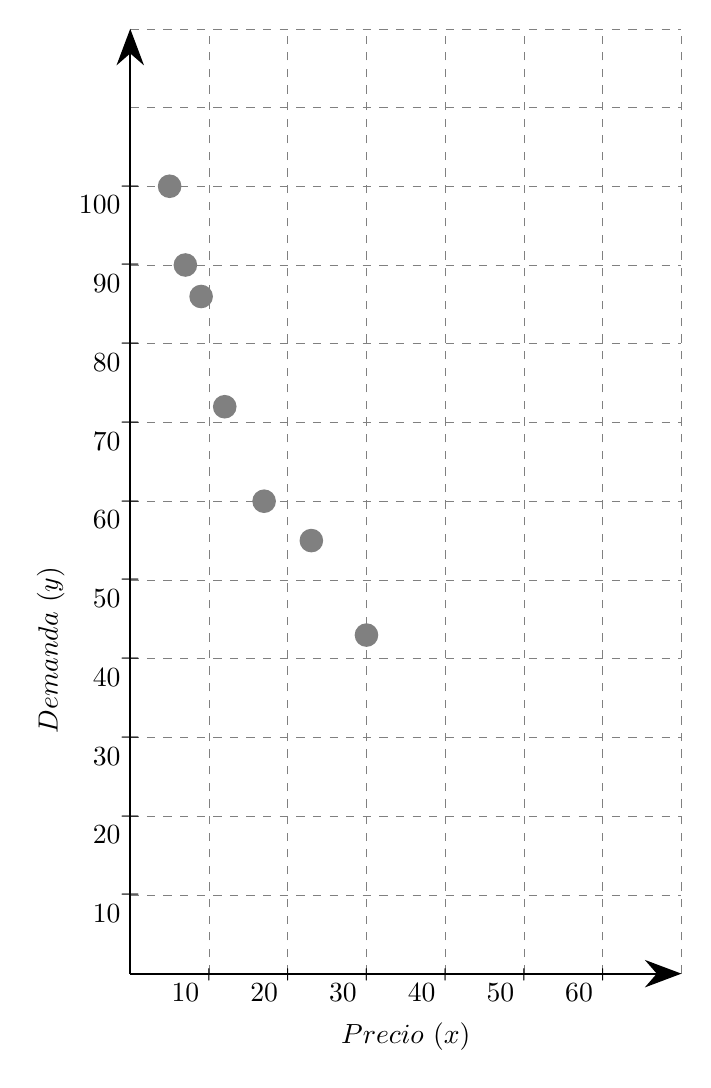
\begin{tikzpicture}
			\draw[step=1,color=blue,help lines,dashed] (0,0) grid (7,12);
			\draw[thick,-{Stealth[scale=2]}] (0,0) -- (7,0) node[rotate=0,midway,below=14pt]{$Precio~(x)$};
			\draw[thick,-{Stealth[scale=2]}] (0,0) -- (0,12) node[rotate=90,midway,above left=20pt]{$Demanda~(y)$};
			\fill[gray] (0.5,10) circle [radius=0.15];
			\fill[gray] (0.7,9) circle [radius=0.15];
			\fill[gray] (0.9,8.6) circle [radius=0.15];
			\fill[gray] (1.2,7.2) circle [radius=0.15];
			\fill[gray] (1.7,6) circle [radius=0.15];
			\fill[gray] (2.3,5.5) circle [radius=0.15];
			\fill[gray] (3,4.3) circle [radius=0.15];
			%numeración eje x
			\node at (1,0) {$\shortmid$};
			\node [below left] at (1,0) {$10$};
			\node at (2,0) {$\shortmid$};
			\node [below left] at (2,0) {$20$};
			\node at (3,0) {$\shortmid$};
			\node [below left] at (3,0) {$30$};
			\node at (4,0) {$\shortmid$};
			\node [below left] at (4,0) {$40$};
			\node at (5,0) {$\shortmid$};
			\node [below left] at (5,0) {$50$};
			\node at (6,0) {$\shortmid$};
			\node [below left] at (6,0) {$60$};
			%numeración eje y
			\node at (0,1) {$-$};
			\node [below left] at (0,1) {$10$};
			\node at (0,2) {$-$};
			\node [below left] at (0,2) {$20$};
			\node at (0,3) {$-$};
			\node [below left] at (0,3) {$30$};
			\node at (0,4) {$-$};
			\node [below left] at (0,4) {$40$};
			\node at (0,5) {$-$};
			\node [below left] at (0,5) {$50$};
			\node at (0,6) {$-$};
			\node [below left] at (0,6) {$60$};
			\node at (0,7) {$-$};
			\node [below left] at (0,7) {$70$};
			\node at (0,8) {$-$};
			\node [below left] at (0,8) {$80$};
			\node at (0,9) {$-$};
			\node [below left] at (0,9) {$90$};
			\node at (0,10) {$-$};
			\node [below left] at (0,10) {$100$};
		\end{tikzpicture}
		\caption{Diagrama de dispersión}
	\end{figure}
	
	Se aprecia que hay una correlación lineal inversa bastante marcada entre los datos suministrados para ambas variables.
	
	\section*{c) Calcular el coeficiente de correlación $\Upsilon$  analizarlo e interpretarlo.}
	\begin{table}[h]
		\centering
		\begin{tabular}{|c|c|c|c|c|c|c|}
			\hline
			$x$ & $y$ & $x-\bar{x}$ & $y-\bar{y}$ & $(x-\bar{x})^2$ & $(y-\bar{y})^2$ & $(x-\bar{x})(y-\bar{y})$ \\ \hline
			$5$ & $100$ & $-9.71$ & $27.72$ & $94.28$ & $768.39$ & $-269.16$ \\ \hline
			$7$ & $90$ & $-7.71$ & $17.72$ & $59.44$ & $313.99$ & $-136.62$ \\ \hline
			$9$ & $86$ & $-5.71$ & $13.72$ & $32.60$ & $188.23$ & $-78.34$ \\ \hline
			$12$ & $72$ & $-2.71$ & $-0.28$ & $7.3$ & $0.07$ & $0.75$ \\ \hline
			$17$ & $60$ & $2.29$ & $-12.28$ & $5.24$ & $150.79$ & $-28.12$ \\ \hline
			$23$ & $55$ & $8.29$ & $-17.28$ & $68.72$ & $298.59$ & $-143.25$ \\ \hline
			$30$ & $43$ & $15.29$ & $-29.28$ & $233.78$ & $857.31$ & $-447.69$ \\ \hline
			$\sum{103}$ & $\sum{506}$ & $\sum{0.03}$ & $\sum{0.04}$ & $\sum{501.36}$ & $\sum{2577.37}$ & $\sum{-1102.43}$ \\ \hline
		\end{tabular}
	\end{table}
	
	\LARGE{$\Upsilon=\frac{\sum{(x-\bar{x})(y-\bar{y})}}{\sqrt{(\sum{(x-\bar{x})^2})(\sum{(y-\bar{y})^2})}}$} \\ \\
	$\bar{x}=\frac{\sum{x}}{n}=\frac{103}{7}\approx14.71$ \\ \\
	$\bar{y}=\frac{\sum{y}}{n}=\frac{506}{7}\approx72.28$ \\ \\
	\large{$\sum{(x-\bar{x})^2} = 501.36$} \\ \\
	$\sum{(y-\bar{y})^2} = 2577.37$ \\ \\
	$\sum{(x-\bar{x})(y-\bar{y})} = -1102.43$ \\ \\
	\large{$\Upsilon = \frac{-1102.43}{\sqrt{501.36*2577.37}} = -0.969$} \\
	
	\paragraph{Interpretación:} \small{El valor negativo indica que la correlación es inversa (a mayor precio, menores unidades demandadas); y el valor cercano a $-1$ indica que el modelo de regresión lineal se ajusta bien con los datos suministrados.}
	
	\section*{d) Calcular la función de ajuste (Ecuación de Regresión) y graficarla sobre el diagrama. Método de los mínimos cuadrados.}
	
	\begin{table}[h]
		\centering
		\begin{tabular}{|c|c|c|c|}
			\hline
			$x$ & $y$ & $xy$ & $x^2$ \\ \hline
			$5$ & $100$ & $500$ & $25$ \\ \hline
			$7$ & $90$ & $630$ & $49$ \\ \hline
			$9$ & $86$ & $774$ & $81$ \\ \hline
			$12$ & $72$ & $864$ & $144$ \\ \hline
			$17$ & $60$ & $1020$ & $289$ \\ \hline
			$23$ & $55$ & $1265$ & $529$ \\ \hline
			$30$ & $43$ & $1290$ & $900$ \\ \hline
			$\sum{103}$ & $\sum{506}$ & $\sum{6343}$ & $\sum{2017}$ \\ \hline
		\end{tabular}
	\end{table}
	
	\Large{$y=mx+b$},\hspace{10pt}\LARGE{$m=\frac{\sum{xy}-\frac{(\sum{x})(\sum{y})}{n}}{\sum{x^2}-\frac{(\sum{x})^2}{n}}$}, \hspace{12pt}\Large{$n=7$} \\ \\
	$m=\frac{6343-\frac{103*506}{7}}{2017-\frac{(103)^2}{7}}=\frac{6343-7445.428}{2017-1515.571}=\frac{-1102.428}{501.429}=-2.198$ \\ \\
	$b=\bar{y}-m\bar{x} = 72.28-(-2.198*14.71)=104.612$
	
	\begin{figure}[h]
		\centering
		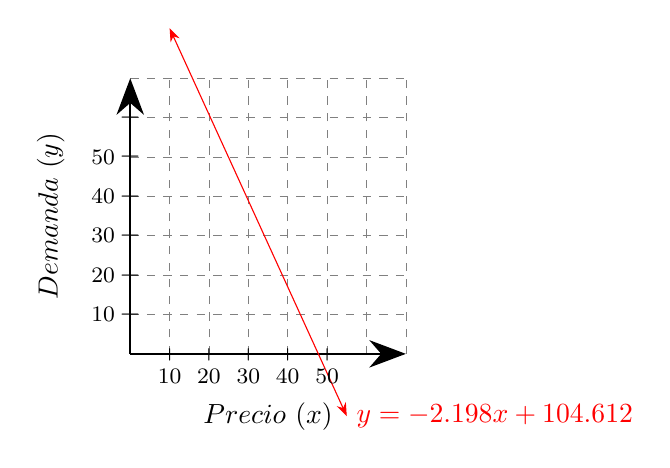
\begin{tikzpicture}[domain=10:55,scale=0.5]
			\draw[step=1,color=gray,help lines,dashed] (0,0) grid (7,7);
			\draw[thick,-{Stealth[scale=2]}] (0,0) -- (7,0)
			node[rotate=0,midway,below=14pt]{$Precio~(x)$};
			\draw[thick,-{Stealth[scale=2]}] (0,0) -- (0,7) node[rotate=90,midway,above=20pt]{$Demanda~(y)$};
			\draw[color=red, Stealth-Stealth] plot (\x/10,{-0.219*(\x)+10.461}) node[right] {$y = -2.198x + 104.612$};
			%numeración eje x
			\node at (1,0) {$\shortmid$};
			\node [below=2pt] at (1,0) {\footnotesize{$10$}};
			\node at (2,0) {$\shortmid$};
			\node [below=2pt] at (2,0) {\footnotesize{$20$}};
			\node at (3,0) {$\shortmid$};
			\node [below=2pt] at (3,0) {\footnotesize{$30$}};
			\node at (4,0) {$\shortmid$};
			\node [below=2pt] at (4,0) {\footnotesize{$40$}};
			\node at (5,0) {$\shortmid$};
			\node [below=2pt] at (5,0) {\footnotesize{$50$}};
			%numeración eje y
			\node at (0,1) {$-$};
			\node [left=2pt] at (0,1) {\footnotesize{$10$}};
			\node at (0,2) {$-$};
			\node [left=2pt] at (0,2) {\footnotesize{$20$}};
			\node at (0,3) {$-$};
			\node [left=2pt] at (0,3) {\footnotesize{$30$}};
			\node at (0,4) {$-$};
			\node [left=2pt] at (0,4) {\footnotesize{$40$}};
			\node at (0,5) {$-$};
			\node [left=2pt] at (0,5) {\footnotesize{$50$}};
			\node at (0,6) {$-$};
		\end{tikzpicture}
		\caption{Ecuación de regresión}
	\end{figure}
	
	\newpage
	
	\section*{e) Pronósticar el precio de venta para 50, 25 y 80 unidades demandadas.}
	$y=-2.198x+104.612$ \\ \\
	$y-104.612=-2.198x$ \\ \\
	$x=\frac{y-104.612}{-2.198}$ \\ \\
	Para $y=50$: \\ \\
	$x=\frac{50-104.612}{-2.198}=\frac{-54.612}{-2.198}=24.846$ \\ \\
	Para $y=25$: \\ \\
	$x=\frac{25-104.612}{-2.198}=\frac{-79.612}{-2.198}=36.220$ \\ \\
	Para $y=80$: \\ \\
	$x=\frac{80-104.612}{-2.198}=\frac{-24.612}{-2.198}=11.197$ \\ \\
	
	\newpage
	
	\section*{f) Pronósticar las cantidades demandadas para un precio de $\$3000$ y $\$120000$.}
	
	Para $x=10$: \\ \\
	$y=-2.198*10+104.612=82.632$ \\ \\
	Para $x=3$: \\ \\
	$y=-2.198*3+104.612=98.018$ \\ \\
	Para $x=120$: \\ \\
	$y=-2.198*120+104.612=-159.148$ \\ \\
	
	\section*{g) Calcular el coeficiente de determinación e interpretar los resultados.}
	
	$\Upsilon^2=(-0.969)^2=0.938$
	\paragraph*{Interpretación de resultados:} \small{El valor del coeficiente de determinación es cercano a $1$. Indicando que el modelo si puede explicar los resultados observados.}
	
	\section*{h) Sacar conclusiones y sugerencias a partir de los resultados obtenidos a travez de este modelo.}
	
	\small{El modelo de regresión se ajusta bien con los datos históricos y se considera un modelo válido para hacer pronósticos.}
	
	
	\section*{Gráfico completo} Diagrama de dispersión y gráfica de la ecuación de regresión.
	\begin{table}[h]
		\centering
		\begin{tabular}{|c|c|c|c|c|c|c|c|c|c|c|c|c|c|}
			\hline
			$x$ & $5$ & $7$ & $9$ & $12$ & $17$ & $23$ & $30$ & $10$ & $24.846$ & $3$ & $36.220$ & $11.97$ & $120$ \\ \hline
			$y$ & $100$ & $90$ & $86$ & $72$ & $60$ & $55$ & $43$ & $82.632$ & $50$ & $98.018$ & $25$ & $80$ & $-159.148$ \\ \hline
		\end{tabular}
	\end{table}
	\begin{figure}[h]
		\centering
		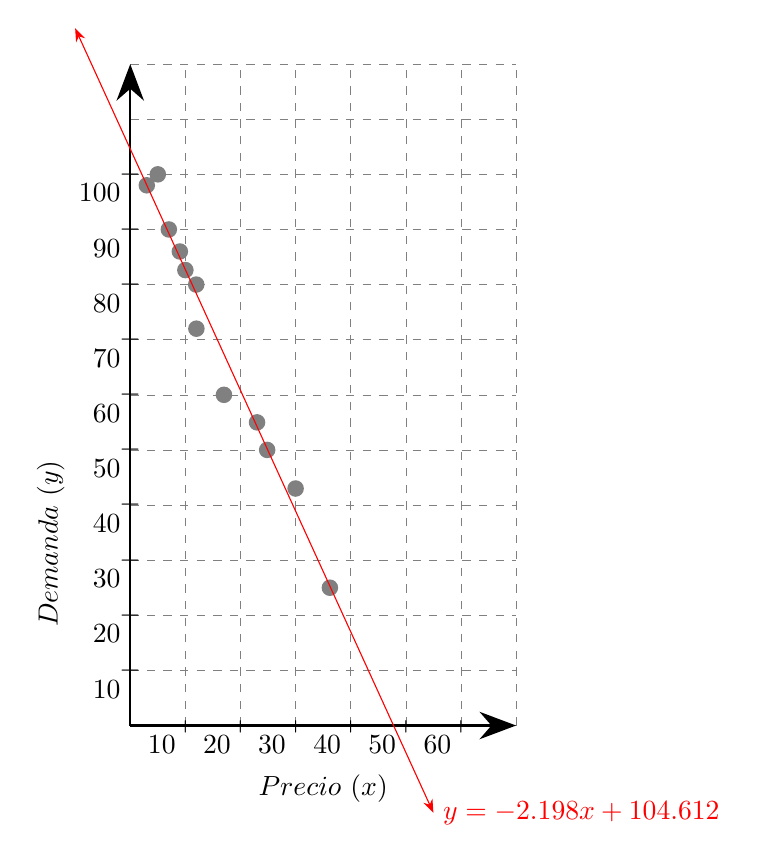
\begin{tikzpicture}[domain=-10:55,scale=0.7]
			\draw[step=1,color=gray,help lines,dashed] (0,0) grid (7,12);
			\draw[thick,-{Stealth[scale=2]}] (0,0) -- (7,0) node[rotate=0,midway,below=14pt]{$Precio~(x)$};
			\draw[thick,-{Stealth[scale=2]}] (0,0) -- (0,12) node[rotate=90,midway,above left=20pt]{$Demanda~(y)$};
			\fill[gray] (0.5,10) circle [radius=0.15];
			\fill[gray] (0.7,9) circle [radius=0.15];
			\fill[gray] (0.9,8.6) circle [radius=0.15];
			\fill[gray] (1.2,7.2) circle [radius=0.15];
			\fill[gray] (1.7,6) circle [radius=0.15];
			\fill[gray] (2.3,5.5) circle [radius=0.15];
			\fill[gray] (3,4.3) circle [radius=0.15];
			\fill[gray] (1,8.263) circle [radius=0.15];
			\fill[gray] (2.484,5) circle [radius=0.15];
			\fill[gray] (0.3,9.801) circle [radius=0.15];
			\fill[gray] (3.622,2.5) circle [radius=0.15];
			\fill[gray] (1.197,8) circle [radius=0.15];
			\draw[color=red, Stealth-Stealth] plot (\x/10,{-0.219*(\x)+10.461}) node[right] {$y = -2.198x + 104.612$};
			%numeración eje x
			\node at (1,0) {$\shortmid$};
			\node [below left] at (1,0) {$10$};
			\node at (2,0) {$\shortmid$};
			\node [below left] at (2,0) {$20$};
			\node at (3,0) {$\shortmid$};
			\node [below left] at (3,0) {$30$};
			\node at (4,0) {$\shortmid$};
			\node [below left] at (4,0) {$40$};
			\node at (5,0) {$\shortmid$};
			\node [below left] at (5,0) {$50$};
			\node at (6,0) {$\shortmid$};
			\node [below left] at (6,0) {$60$};
			%numeración eje y
			\node at (0,1) {$-$};
			\node [below left] at (0,1) {$10$};
			\node at (0,2) {$-$};
			\node [below left] at (0,2) {$20$};
			\node at (0,3) {$-$};
			\node [below left] at (0,3) {$30$};
			\node at (0,4) {$-$};
			\node [below left] at (0,4) {$40$};
			\node at (0,5) {$-$};
			\node [below left] at (0,5) {$50$};
			\node at (0,6) {$-$};
			\node [below left] at (0,6) {$60$};
			\node at (0,7) {$-$};
			\node [below left] at (0,7) {$70$};
			\node at (0,8) {$-$};
			\node [below left] at (0,8) {$80$};
			\node at (0,9) {$-$};
			\node [below left] at (0,9) {$90$};
			\node at (0,10) {$-$};
			\node [below left] at (0,10) {$100$};
		\end{tikzpicture}
	\end{figure}
\end{document}